% !TEX encoding = UTF-8 Unicode

\documentclass[a4paper]{article}

\usepackage{color}
\usepackage{url}
\usepackage[T2A]{fontenc} % enable Cyrillic fonts
\usepackage[utf8]{inputenc} % make weird characters work
\usepackage{graphicx}
\graphicspath{ {slike/} }



\usepackage[english,serbian]{babel}
%\usepackage[english,serbianc]{babel} %ukljuciti babel sa ovim opcijama, umesto gornjim, ukoliko se koristi cirilica

\usepackage[unicode]{hyperref}
\hypersetup{colorlinks,citecolor=green,filecolor=green,linkcolor=blue,urlcolor=blue}

%\newtheorem{primer}{Пример}[section] %ćirilični primer
\newtheorem{primer}{Primer}[section]

\begin{document}

\title{Verifikacija softvera\\ \small{Seminarski rad u okviru kursa\\Metodologija stručnog i naučnog rada\\ Matematički fakultet}}

\author{Peleksić Ljubica, Milica Kojičić \\ peleksic.ljubica@gmal.com, milicakojicic@gmail.com}
\date{31.~mart 2015.}
\maketitle

\abstract{


\tableofcontents

\newpage

\section{Uvod}
\label{sec:uvod}






\section{Simboličko izvršavanje}
\label{sec:naslov1}
U ovom odeljku ćemo se baviti simboličkim izvršavanjem programa. Radi se o tome da se umesto prosleđivanja normalnog ulaza programu, prosleđuju proizvoljne simboličke vrednosti. Izvršavanje programa se odvija normalno, osim što vrednosti mogu biti proizvoljne formule sastavljenje od ulaznih simbola. Teški, ali i zanimljivi problemi koji nastaju pri simboličkom izvršavanju, potiču od uslovnih grananja. Proizvodnja velikih razmera pouzdanih programa je jedan od osnovnih uslova za primenu računara u izazovnim problemima današnjice. Neke tehnike se koriste u praksi, a neke su još uvek tema istraživanja. Program treba da ispunjava zahteve, iako nisu date formalne specifikacije. Neki uzorak podataka koji treba da bude obrađen od strane programa je dat programu. Ako je ocenjeno da program proizvodi korektan rezultat za dati uzorak podataka, pretpostavlja se da je on i tačan. Osnovno pitanje koje se postavlja je kako odabrati taj uzorak.

Skorašnji radovi o dokazivanju korektnosti programa formalnom analizom obecavaju mnogo i pokazuje se da je to ultimativna tehnika za pravljenje pouzdanih programa. Ali nije verovatno da će se svođenje teorije na praksu lako rešiti u skoroj budućnosti. Testiranje programa i dokazivanje korektnosti programa mogu se posmatrati kao ekstremne alternative. Dok testira, programer može biti siguran da za neki test primer u uzorku program radi tačno pažljivim proučavanjem rezultata. Tačnost izvršavanja za ulaze koji nisu u uzorku je i dalje podložan sumnji. S druge strane, pri dokazivanju korektnosti programa, programer formalno dokazuje da program pri svakom izvršavanju ispunjava zahteve koji su dati specifikacijom, a da pritom ne mora da izvršava program uopšte. Da bi to mogao, on daje preciznu specifikaciju tačnog ponašanja programa i dalje sledi formalnu proceduru dokazivanja da bi pokazao da su program i specifikacija konzistentni. Poverenje u ovaj metod zavisi od tačnosti pri kreiranju specifikacije i konstrukcije koraka u dokazu, kao i od mašinski zavisnih problema kao što su prekoračenje, zaokruživanje itd...  Ovde se radi o praktičnom pristupu između ove dve krajnosti. Iz najprostijeg ugla, ovo je poboljšana vrsta tehnike testiranja. Umesto izvršavanja programa nad skupom ulaza, program se ''simbolično'' izvršava nad klasama ulaza. To znači da rezultat simboličkog izvršavanja može biti ekvivalentan velikom broju uobičajenih test primera. I ovi rezultati svakako mogu biti provereni od strane programera. Klasa ulaza, okarakterisana svakim simboličkim izvršavanjem, je određena u zavisnosti od kontrole toka programa nad ulazom. Ako je kontrola toka programa u potpunosti nezavisna od ulaznih varijabli, jedno simboličko izvršavanje će biti dovoljno da proveri sva moguća izvršavanja programa. Ako pak, kontrola toka zavisi od ulaza, mora se pribeći analizi slučajeva. Često, skup ulaznih klasa je koji pokrivaju sve moguće slučajeve je praktično beskonačan, tako da je ovo i dalje metoda testiranja. Kako god, ulazne klase su određene samo onim ulazima koji utiču na kontrolu toka i simboličko testiranje obećava postizanje boljih rezultata mnogo lakše od običnog testiranja.  


U nastavku ćemo se baviti simboličkim izvršavanjem u idealnom smislu, idealnom iz sledećih razloga:
Pretpostavka je da programi obrađuju samo cele brojeve proizvoljne veličine. Drveta izvršavanja koji su rezultat simboličkog izvršavanja su za većinu programa beskonačna. Takođe, simboličko izvršavanje \textit{IF} naredbe zahteva dokazivanje teorema, što je za jednostavnije programske jezike praktično nemoguće ostvariti. Ovaj idealni sistem nam predstavlja standard u odnosu na koji se sistemi za simboličko izvršavanje mogu meriti. Svaki programski jezik ima svoju semantiku izvršavanja, koja opisuje kakve podatke varijable mogu da reprezentuju, kako naredbe manipulišu tim podacima i kojim se tokom odvija  izvršavanje naredbi. Paralelno se može definisati alternativna semantika simboličkog izvršavanja, u kojoj se pravi podaci ne koriste, ali mogu biti predstavljeni proivoljnim simbolima. Simboličko izvršavanje predstavlja prirodnu ekstenziju normalnog izvršavanja, u kojoj su operatori programskog jezika prošireni tako da prihvataju simboličke ulaze i proizvode simboličke formule na izlazu. Pritom, semantika izvršavanja je promenjena u smislu da podržava simboličko izvršavanje, ali ni sintaksa jezika, ni pojedinačni programi pisani u tom jeziku nisu promenjeni. Jedini način da se simbolički podaci predstave programu jeste da mu se daju kao ulaz. Svaki put kada program zahteva novu ulaznu vrednost, ona mu se obezbeđuje iz liste simbola \{$\alpha_1, \alpha_2, \alpha_3, ... $ \}. Oni će u nekom trenutku biti dodeljeni kao vrednosti programskim varijablama (kao parametri procedura, globalne varijable i slično). Da bismo mogli da baratamo simboličkim ulazima, dozvoljeno je da vrednosti varijabli mogu da budu $\alpha_i$, kao i celobrojne konstante. I aritmetički izrazi, kao i \textit{IF} naredbe moraju biti proširene tako da mogu da barataju sa simboličkim vrednostima. Time što dozvoljavamo da varijable uzimaju vrednosti polinoma nad $\alpha_i$, simboličko izvršavanje naredbi dodele teče prirodno.
Stanje izvršavanja programa obično uključuje vrednosti varijabli, kao i brojač instrukcija, koji nam daje informaciju o tome koja se naredba trenutno izvršava. Definicija simboličkog izvršavanja \textit{IF} naredbe zahteva da se u stanje izvršavanja uključi i uslov putanje (path condition - \textit{pc}). \textit{Pc} predstavlja logički izraz nad simboličkim ulazima \{$\alpha_i$\}. On nikad ne sadrži programske varijable, i možemo ga predstaviti u obliku konjukcije izraza forme $R \ge 0$ ili  $\neg(R \ge 0)$, gde je\textit{R} polinom nad \{$\alpha_i$\}. Na primer:  \{$\alpha_1 > 0 \wedge  \alpha_2 + 3 > 0 $\}. Kao što ćemo videti \textit{pc} predstavlja akumulator osobina koje ulaz mora da zadovolji da bi izvršavanje pratilo određenu pridruženu putanju. Svako simboličko izvršavanje počinje tako što se \textit{pc} inicijalizuje na tačno. Kako se prave pretpostavke o ulazima, u cilju odabira putanje koja je odredjena \textit{IF} naredbom, te pretpostavke se dodaju u \textit{pc}. Simboličko izvršavanje \textit{IF} naredbe teče kao njeno normalno izvršavanje, evaluacijom njoj pridruženog logičkog izraza 
zamenjivanjem varijabli njihovim vrednostima. Kako su vrednosti varijabli polinomi nad \{$\alpha_i$\}, uslovni izraz je u formi $R \ge 0$, gde je \textit{R} polinom. Nazovimo taj izraz \textit{q}. Koristeći trenutni \textit{pc}, formiramo sledeće izraze: \\
(a) $pc \supset q$ \\  
(b) $pc \supset \neg q $ \\
Najviše jedan od ova dva tvrđenja mođe biti tačan (eliminišemo trivijalan slučaj kad je \textit{pc} netačan). Kada je tačno jedan od ova dva izraza tačan, nastavlja se sa izvršavanjem \textit{IF} naredbe tako što se kontrola toka prebacuje na njen \textit{THEN} deo ako je izraz (a) tačan ili na njen \textit{ELSE} deo ako je (b) tačno. Ovakav tip izvršavanja se zove ne račvajući, jer se izvršava tačno jedna od sve grane, za razliku od slučaja kada ni slučaj (a) ni slučaj (b) nisu tačni. U ovakvoj situaciji postoji skup ulaza u program koji zadovoljava pc i koji bi pratio \textit{THEN} alternativu, ali postoji i skup ulaza koji bi išao \textit{ELSE} alternativom. Pošto su obe alternative moguće, jedini kompletan pristup bi bio da se ispitaju obe putanje, tako da se ovde simboličko izvršavanje "račva" u dve putanje. Biranjem \textit{THEN} alternative, pretpostavlja se da ulazi zadovoljavaju \textit{q}, pa je ta informacija dodata u \textit{pc} : $ pc \gets pc \wedge q $. Isto tako, biranjem \textit{ELSE} alternative dobijamo 
$ pc \gets pc \wedge \neg q $. \textit{Pc} se zove "putanja uslova" jer predstavlja akumulaciju uslova koji određuju jedinstvenu kontrolu toka u programu.

\subsection{Drvo izvršavanja}
Drvo izvršavanja opisuje putanje kojima je teklo simboličko izvršavanje programa. Svakom čvoru drveta je priključena izvršena naredba (označena brojem), dok svaka veza između čvorova predstavlja direktnu vezu između naredbi. Za svako račvajuće izvršavanje \textit{IF} naredbe od odgovarajućeg čvora polaze dve veze koje su označene sa "T" i "F" za tačan (\textit{THEN}) i netačan (\textit{ELSE}) deo, respektivno. Takođe se svakom čvoru pridružuju vrednosti varijabli, brojač instrukcija, kao i \textit {pc}. Simbolička izvršavanja za funkciju koja izračunava stepen broja su data na \textit {Slici 1.}

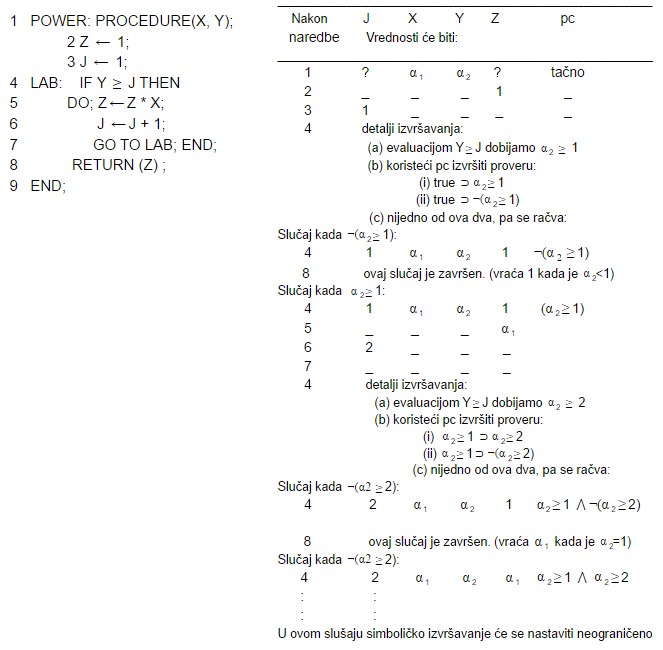
\includegraphics[width=0.7\textwidth]{Slika1}

\textit{Slika 1}

Drveta formirana na ovaj način imaju sledeće zanimljive osobine:
Za svaki terminalni čvor (koji odgovara kompletno izvršenoj putanji) u drvetu postoji odgovarajući nesimbolički ulaz u program, koji će tokom normalnog izvršavanja programa pratiti istu putanju (listu izvršenih naredbi), što je ekvivalentno tvrđenju  da \textit{pc} nikad neće postati netačno. Druga važna osobina jeste da je u u svakom terminalnom čvoru vrednost \textit{pc}-ja jedinstvena. Dve putanje koje polaze iz zajedničkog korena drveta odlučivanja imaju jedinstven čvor račvanja, odakle putanje pocinju da divergiraju, u smislu da je u tom čvoru jednom \textit{pc}-ju dodat neki \textit{q} a drugom $\neg q$. Posto u tom slučaju pc neće postati netačno, oni moraju da se razlikuju. 

\subsection{Komutativnost}

Ovako definisano simboličko izvršavanje zadovoljava osobinu komutativnosti. Naime, ako se program izvršava na konvencionalni način, sa određenim skupom celobrojnih vrednosti \{$j_i$\} na ulazu (dakle prvo se izvrši operacija instanciranja simbola \{$\alpha_i$\} specifičnim celobrojnim vrednostima), rezultat će biti isti ako prvo izvršimo program simbolički, pa onda instanciramo simboličke rezultate (dodelimo $j_i$ $\alpha_i$), što se vidi i na slikama iznad. Upravo je ova osobina komutativnosti simboličkog izvršavanja od značaja. Ono proizvodi iste efekte kao i konvencionalno izvršavanje i nije proizvoljna alternativa, već prirodna ekstenzija normalnom izvršavanju programa.

\subsection{Simboličko izvršavanje i dokazivanje korektnosti programa}
\label{subsec:podnaslovN}


Pri dokazivanju korektnosti programa, programer uz sam program podrazumeva i "ulazni" i "izlazni" predikat koji  definišu tačno ponašanje programa. Program je korektan ako za sve ulaze koji zadovoljavaju ulazni predikat, rezultati koji proizilaze iz izvršavanja programa (ako ih uopšte ima) zadovoljavaju izlazni predikat. Jedan od koraka pri dokazivanju korektnosti programa - \textit{generisanje uslova verifikacije}, se poprilično lako može uraditi simboličkim izvršavanjem programa.

Simboličko izvršavanje je takođe korisno i u drugim aspektima programske analize, uključujući i generisanje test primera kao i u optimizaciji programa. Pretpostavimo da imamo dodatne tri naredbe \textit{ASSERT}, \textit{PROVE} i \textit{ASSUME} koje se koriste da povežu predikat sa programom. Sve tri naredbe imaju kao argumente logičke izraze, npr: \textit{ASSERT(X>0)}. Varijable u ovim formulama su programske varijable i ako pretpostavimo da je B argument ovih naredbi, onda se on evaluira koristeći trenutne vrednosti programskih varijabli i rezultujuća vrednost se dodaje \textit{pc}-ju: $pc \gets pc \wedge value (B)$. Naredba \textit{PROVE(B)} se izvršava, formira izraz $pc \supset value(B)$ i pokušava da dokaže da je to teorema. Pored prethodno navedena dva predikata, mogu se definisati i dodatni induktivni predikati(u svakoj petlji najmanje jedan predikat npr.). Predikati su povezani sa programom koristeći \textit{ASSERT} naredbu (inicijalni predikat je \textit{ASSERT} naredba na početku programa). I sada imamo fiksiran skup putanja kroz program gde svaki od njih počinje i završava se sa \textit{ASSERT} i za svaki mora da se dokaže njegova korektnost. Dokaz korektnosti svake putanje dokazuje se njenim simboličkim izvršavanjem i to:

\begin{enumerate}
\item {Menjanjem \textit{ASSERT} naredbe na početku sa \textit{ASSUME}, kao i menjanjem iste naredbe sa \textit{PROVE} na kraju.}  
\item{ Inicijalizovanjem pc-ja na tačno i programske varijable na $\alpha_1, \alpha_2 $, ... }
\item { Simboličkim zvršavanjem date putanje }
\item {Ako \textit{PROVE} na kraju putanje pokaže tačno, putanja je korektna, a inače nije }
 \end{enumerate}
Pošto simboličko izvršavanje zadovoljava svojstvo komutativnosti, jednostavno je zaključiti da je ovo validan metod dokazivanja. Izvršavanjem \textit{PROVE} na kraju putanje postavlja kandidata za teoremu: dakle, ako pretpostavimo da je predikat na početku bio zadovoljen i mi smo pratili ovu putanju koja je snimljena u \textit{pc}-ju, pitamo se da li trenutne vrednosti programa na kraju ove konkretne putanje zadovoljavaju predikat na kraju. Usvajajući ovakvu definiciju za \textit{PROVE} naredbu za dokazivanje korektnosti, je vrlo korisno i za tesitiranje korektnosti metodom simboličkog izvršavanja. Naime, u testiranju programa (bilo ono simboličko ili ne) moraju da se ispituju izlazi iz programa i mora da se sudi o njihovoj korektnosti.  Ako kriterijum korektnosti može da se formalizuje u smislu ulaznog i izlaznog predikata, onda simbolički izvršilac nakon toga takođe može da pouzdano proveri test rezultate. Za svaki program čije je simboličko drvo konačno i kod koga je kriterijum korektnosti eksplicitno zadat ulaznim i izlaznim predikatima, iscrpno simboličko izvršavanje i dokazivanje korektnosti su zapravo isti proces.


 
\section{Drugi naslov}
\label{sec:naslov2}






\subsection{... podnaslov}
\label{subsec:podnaslovK}


\subsection{... podnaslov}
\label{subsec:podnaslovM}


\section{Poslednji naslov}
\label{sec:naslovM}


\section{Zaključak}
\label{sec:zakljucak}

\addcontentsline{toc}{section}{Literatura}
\appendix
\bibliography{seminarski} 
\bibliographystyle{plain}

\appendix
\section{Dodatak}


\end{document}
